\documentclass[11pt]{article}
\usepackage{amssymb, latexsym, mathtools, amsthm}
\pagestyle{plain}
\begingroup
    \makeatletter
    \@for\theoremstyle:=definition,remark,plain\do{\expandafter\g@addto@macro\csname th@\theoremstyle\endcsname{\addtolength\thm@preskip\parskip
            }}
\endgroup
\usepackage{pgf,tikz}
\usepackage{pdfsync}
\usepackage{txfonts}
\usepackage[T1]{fontenc}
\usepackage{booktabs}
 \usepackage{graphicx}
\definecolor{dnrbl}{rgb}{0,0,0.3}
\definecolor{dnrgr}{rgb}{0,0.3,0}
\definecolor{dnrre}{rgb}{0.5,0,0}
\usepackage[colorlinks=true, citecolor=dnrgr, linkcolor=dnrre, urlcolor=dnrre] {hyperref}
\usepackage{xcolor}
\usepackage{parskip}
\usepackage{tabularx, colortbl}
\usepackage{geometry}
 \geometry{
 left=26mm,
 right=26mm,
 top=26mm,
 bottom=26mm,  footskip=1cm} 

 \usepackage[scriptsize, up]{caption}
\usepackage{pgf,tikz}
\usetikzlibrary{decorations, decorations.pathmorphing}
\usetikzlibrary {shapes}
\newcommand*{\ditto}{------\raisebox{-0.5ex}{\textquotedbl}------\ \ }




\setcounter{totalnumber}{1}
\setcounter{topnumber}{1}
\setcounter{bottomnumber}{0}


\theoremstyle{plain}
\newtheorem{thm}{Theorem}[section]
\newtheorem{prop}[thm]{Proposition}
\newtheorem{lem}[thm]{Lemma}
\newtheorem{coro}[thm]{Corollary}
\newtheorem{defi}[thm]{Definition}
\numberwithin{equation}{subsection}
\makeatletter
\renewcommand*{\thetable}{\arabic{table}}
\renewcommand*{\thefigure}{\arabic{figure}}
\let\c@table\c@figure
\makeatother 
\def\proofname{{\bf Proof.}}
\def\datename{{\em This version:}}
\newcommand{\into}{\searrow}
\newcommand{\Nat}{\mathbb{N}}
\newcommand{\Real}{{\mathbb R}}
\newcommand{\Rat}{{\mathbb Q}}
\newcommand{\restr}{\upharpoonright}  \newcommand{\un}{\uparrow} \newcommand{\de}{\downarrow} \DeclarePairedDelimiter{\ceil}{\lceil}{\rceil}
\DeclarePairedDelimiter{\floor}{\lfloor}{\rfloor}
\newcommand{\la}{\langle}
\newcommand{\ra}{\rangle}
\newcommand{\bigo}[1]{\mathop{\bf O}\/\left({#1}\right)}
\newcommand{\smo}[1]{\mathop{\bf o}\/\left({#1}\right)}
\newcommand{\ZZ}{\mathbf{Z}}
\newcommand{\DD}{\mathbf{D}}
\newcommand{\GG}{\mathbf{G}}
\newcommand{\FF}{\mathbf{F}}
\newcommand{\XX}{\mathbf{X}}
\newcommand{\YY}{\mathbf{Y}}
\newcommand{\CC}{\mathbf{C}}
\newcommand{\TT}{\mathbf{T}}
\newcommand{\LL}{\mathbf{L}}
\newcommand{\II}{\mathbf{I}}
\newcommand{\JJ}{\mathbf{J}}
\newcommand{\pp}{\mathbf{p}}

\newcommand{\neig}[1]{\mathcal{N}(#1)}
\newcommand{\bias}[1]{\mathtt{B}(#1)}
\newcommand{\mix}{\textsc{mix}}
\newcommand{\unhap}{\mathtt{U}}
\newcommand{\blocka}{\mathtt{k}_{\alpha}}
\newcommand{\blockb}{\mathtt{k}_{\beta}}
\newcommand{\Punhap}{\mathbb{P}_{\textrm{unhap}}}
\newcommand{\Pstab}{\mathbb{P}_{\textrm{stab}}}
\DeclareRobustCommand{\expo}[2][{\mbox{}}]{\ensuremath {#1}\left( {#2} \right)}
\DeclareRobustCommand{\expe}[2][{\mbox{}}]{\ensuremath {#1}\left[ {#2} \right]}
\DeclareRobustCommand{\expec}[3][{\mbox{}}]{\ensuremath {#1}\left[ {#2} \ \big|\  {#3} \right]}
\DeclareRobustCommand{\expeco}[4][{\mbox{}}]{\ensuremath {#1}_{#4}\left[{#2} \ \big|\  {#3} \right]}
\DeclareRobustCommand{\proba}[2][{\mbox{}}]{\ensuremath {#1} [ {#2} ]}
\DeclareRobustCommand{\probac}[3][{\mbox{}}]{\ensuremath {#1}[ {#2} \ |\  {#3} ]}






\renewenvironment{abstract}
 { \normalsize
  \list{}{
    \setlength{\leftmargin}{.0cm}\setlength{\rightmargin}{\leftmargin}}\item {\bf \abstractname.} \relax}
 {\endlist}
\title{Minority
population in the one-dimensional 
Schelling  model of segregation
\thanks{Authors are listed alphabetically. 
Barmpalias was supported by the 
1000 Talents Program for Young Scholars from the Chinese Government,
and the Chinese Academy of Sciences (CAS) President's International 
Fellowship Initiative No. 2010Y2GB03.
Additional support was received by
the CAS and the Institute of Software of the CAS.
Partial support was also received from a Marsden grant of New Zealand 
and the China Basic Research Program (973) grant No.~2014CB340302.
Lewis-Pye was supported by a Royal Society University 
Research Fellowship. We would like to thank Pan Peng and Zhang Wei 
from the Institute of Software of the CAS, for helpful discussions.}}

\author{George Barmpalias  \and Richard Elwes \and	Andy Lewis-Pye}
\date{\today}
\begin{document}

\maketitle


\begin{abstract}
The Schelling model of segregation looks to explain the way in which a population of agents or particles of two types may come to organise itself into large homogeneous clusters, and can be seen as a variant of the Ising model in which the system is subjected to rapid cooling.  
While the model has been very extensively studied, the unperturbed (noiseless) version has largely resisted rigorous analysis, with most results in the literature pertaining to versions of the model in which noise is introduced into the dynamics so as to make it amenable to standard techniques from statistical mechanics or stochastic evolutionary game theory. 

We rigorously analyse the one-dimensional version of the model in 
which one of the two types is in the minority, and establish various forms of threshold behaviour. 
 Our  results are in sharp contrast with the case when the distribution of the two types
is uniform (i.e.\ each agent has equal chance of being of each type in the initial configuration), which was studied in
\cite{brandt:an, BELschel13}. 
\end{abstract}
\vspace*{\fill}
\noindent{\bf George Barmpalias}\0.2em] 
\textit{E-mail:} \texttt{\textcolor{dnrgr}{barmpalias@gmail.com}}.
\textit{Web:} \texttt{\textcolor{dnrre}{http://barmpalias.net}}\par
\addvspace{\medskipamount}
\noindent{\bf Richard Elwes}\0.2em]
\textit{E-mail:} \texttt{\textcolor{dnrgr}{r.h.elwes@leeds.ac.uk.}}
\textit{Web:} \texttt{\textcolor{dnrre}{http://richardelwes.co.uk}}\par
\addvspace{\medskipamount}
\noindent{\bf Andy Lewis-Pye}\0.2em]
\textit{E-mail:} \texttt{\textcolor{dnrgr}{A.Lewis7@lse.ac.uk.}}
\textit{Web:} \texttt{\textcolor{dnrre}{http://aemlewis.co.uk}} 
\vfill \thispagestyle{empty}
\clearpage
\section{Introduction}
The economist Thomas Schelling introduced his model of segregation in 
 \cite{TS1} (developed later in \cite{TS71a, TS71b}), with the explicit intention of 
 explaining the phenomenon of
racial segregation in large cities. 
Perhaps the earliest 
agent-based model studied by economists, since then it has become 
an archetype of agent-based modelling, prominently
featuring in libraries of modelling software tools such as NetLogo \cite{NetLogo}
and often being the subject of 
experimental analysis and simulations in the modeling and AI communities 
\cite{MF, howtop, FMpref, Gilbert14052002, Martijn2007, yilmaz2009agent, heppenstall2011agent, 
deSmith:2007:GAC:1557282, epstein1996growing}.
Many versions of the model have been analysed theoretically, from
a number of different viewpoints and disciplines: statistical mechanics
\cite{DM, RevModPhys.81.591} and \cite[Section 3.1]{Bertin}, 
evolutionary game theory \cite{HY, JZ1, JZ2, JZ3}
the social sciences \cite{CF, Clarkdem, SandSDo}, and more recently
computer science and AI \cite{CACP07, DBLP:conf/soda/BhaktaMR14, brandt:an, BELschel13}. 
It was observed in \cite{brandt:an}, however,  that despite the vast amount of work that has been
done on the Schelling model in the last 40 years, rigorous mathematical analyses in the previous  literature generally 
concern altered versions of the model, in which noise is introduced in the dynamics, i.e.\ where
one allows that agents may make non-rational decisions that are
detrimental to their welfare with small probability.
The introduction of such `perturbations' may be justifiable from a
`bounded rationality' standpoint. 

The model (which will be formally defined shortly) concerns a population of agents arranged geographically, each being of one of two types. Each agent has a certain neighbourhood around them that they are concerned with, and also an intolerance parameter  which we shall assume here to be the same for all agents. An agent's behaviour is dictated by the proportion of the agents in their neighbourhood which are of its own type. So long as  this proportion is  the agent may be considered `happy' and will not move.  Starting with a random configuration,  one then considers a discrete time dynamical process.  At each stage unhappy agents  may be  given the opportunity to move, swapping positions with another agent,  so as to increase the proportion of their own type within their neighbourhood. Now one might  justify  a perturbed version of these dynamics,  in which  agents will occasionally move in such a way as to decrease their utility (i.e.\  the  proportion of their own type within their neighbourhood) by arguing, for example, that it is reasonable to suppose that only incomplete information about the make-up of each neighbourhood is available to the agents. 
It is a fact, however,  that 
\begin{itemize}
\item[(a)] the methods used for the analysis of
the perturbed models do not apply to the unperturbed model; 
\item[(b)] the segregation that occurs in the perturbed models is often very
different than in the unperturbed model.
\end{itemize}
In the unperturbed models the underlying 
Markov chain does not have the regularities that are found in the perturbed case
(e.g.\ the Markov process is irreversible).  The presence of a large variety of absorbing states means that entirely different and more combinatorial methods are now required. Beyond the basic aim of a rigorous analysis for these unperturbed models, which have been so extensively studied via simulations, further motivation is provided by the fact that the Schelling model is part of a large family of models, arising in a broad variety of contexts---spin glass models, Hopfield nets, cascading phenomena as studied by those in the networks community---all of which look to understand the discrete time dynamics of competing populations on underlying network structures of one kind or another,  and for many of which the unperturbed dynamics are of significant interest.  The hope is that techniques developed in analysing  unperturbed Schelling segregation may pave the way for similar analyses in these variants of the model.  

The first rigorous analysis of an 
unperturbed Schelling model was described 
by  Brandt, Immorlica, Kamath, and Kleinberg
in \cite{brandt:an}. 
In this work it was also demonstrated that the eventual state of the 
process differs significantly from the stochastically stable states of the perturbed models.
This study focused on the one-dimensional Schelling model 
and provided an asymptotic analysis, in the sense that the results hold 
with arbitrarily high probability
for all sufficiently
large neighbourhoods and population.
More significantly, however, it dealt only with the symmetric case where
intolerance parameter   (i.e.\ an agent is happy when at least 50\% of the agents
in its neighbourhood are of its own type). 
 In  \cite{BELschel13}
a much more general analysis of the unperturbed one-dimensional Schelling model
for  was provided. In fact it was shown there that various forms of surprising threshold behaviour exist. 
A significant symmetry assumption underlying 
the results in \cite{brandt:an, BELschel13}
is that
the populations of the two types of agents are assumed to be uniform 
(i.e.\ each agent has equal chance of being of each type in the initial configuration). 
Indeed, there is no rigorous study of the unperturbed spacial proximity model with swapping agents
for the rather realistic  case where the distribution of the two types of agents is skewed.
In fact, the question as to what type of segregation occurs with a skewed population distribution
was raised by  Brandt, Immorlica, Kamath, and Kleinberg 
in \cite[Section 4]{brandt:an} as well as in popular expositions
of the Schelling model like \cite{Hayes}.

The purpose of the present work is to give an answer to this question.
We show that complete segregation is the likely outcome if and only if the intolerance
parameter is larger than . Moreover in the case that the minority type is at most 
25\%, there is a dichotomy between complete segregation and almost complete
absence of segregation.

\begin{table}
\caption{Parameters of the Schelling model and the main result.}\label{ta:paraandmainres}
\colorbox{black!10}{\arrayrulecolor{green!50!black}
  \begin{tabular}{lcc}
{\bf\small  Parameter}&  
{\bf\small  Symbol} &{\bf\small  Range} \1ex]
{\small Neighbourhood radius}    \hspace{0.0cm} & {\small } \hspace{0.0cm} &{\small }\1ex]
{\small Expected/Actual minority proportion}  \hspace{0.0cm}  &  {\small /}
\hspace{0.0cm}  & {\small }\1ex]
\toprule
{\small  \hspace{0.1cm}}&{\small\&\hspace{0.2cm}}&
{\small } & \hspace{0.0cm}  & {\small Negligible}\1ex]
{\small }\hspace{0.1cm} &{\small\&\hspace{0.2cm}}& 
{\small } &	\hspace{0.0cm}  & {\small Negligible}\
\parbox{12cm}{\textup{
[ \& ]\hspace{0.5cm}or\hspace{0.5cm}
[ \& ]\hspace{0.5cm}or\hspace{0.5cm}
[ \& ]}
}
1ex]
\toprule
{\small Social welfare}&  {\small } &{\small Positive (strictly  if )} \1ex]
  {\small No.\ of unhappy nodes} &  {\small } &{\small Approximately negative if } \1ex]
 \toprule
{\small } &{\small  }\1ex]
{\small }  &{\small }\0.5ex]
\toprule
{\small Balanced happiness\hspace{0.6cm}}&  {\small , }  
&\hspace{0.6cm}{\small } &\hspace{0.6cm}{\small } \0.1ex]
\end{tabular}}
\centering
\end{table}


\begin{coro}[Phase transition on ]\label{coro:drphasetans}
If , 
then with high probability the process  
\begin{itemize}
\item converges to complete segregation if ;
\item is static, if .
\end{itemize}
Moreover with high probability it 
reaches its final state in time
, if 
and time , if .
\end{coro}

We display these results in the second item of Table \ref{ta:paraandmainres}.
In Sections \ref{se:analyticsche}--\ref{se:casetaubhalf} we present the argument that proves these results.
This argument uses a number of smaller results which are stated without proof, and are the building blocks of
the proof of Theorem \ref{th:complsegm}. It is our intention that the reader gets a fairly good understanding
of our analysis in this part of the paper, without the burden of having to verify some of the more technical
parts of the proof. Section \ref{se:prelim} is an appendix with detailed proofs of all the facts that were used in
Sections \ref{se:analyticsche}--\ref{se:casetaubhalf}, and completes the proofs of Theorem \ref{th:complsegm} and
Corollary \ref{coro:drphasetans}.

Our proof of Theorem 
is nonuniform, and the analysis is roughly divided in the two cases displayed in Table \ref{ta:validptwocasesnadcorr}:
{\em balanced and unbalanced happiness}. Here {\em happiness} refers to the numbers of initially happy nodes of the
two types, and determines the dynamics that drives the process to an equilibrium. Of the two cases, 
{\em unbalanced happiness} is the most challenging to deal with, and the dynamics is driven by small number of unhappy
-nodes against the large number of unhappy -nodes, which in fact is preserved throughout a significant part of the process.
 

\section{Metrics and reaching complete segregation}\label{se:analyticsche}
One of the most challenging problems in the analysis of the segregation process
is the large number of absorbing states. In order to understand which transitions are possible,
we use certain metrics that 
describe the current state.


\begin{figure}
\includegraphics[scale=0.32]{./skewedpic.png}
\centering
 \caption{The first plot is
from the process 
and the second one 
from the process .
These simulations illustrate that the number -nodes in the infected area remains bounded, until
the number of -nodes outside the infected area becomes small. The second figure also illustrates
the fact that the number of unhappy nodes fluctuates locally.}\label{fig:inf_area}
\end{figure}  


\subsection{Welfare, mixing, and expectations}
We define
global metrics that reflect the welfare of the entire population. An obvious choice
is the number of happy nodes at a given state. It is not hard to devise 
transitions of the process which reduce the total number of happy nodes 
(see the second plot of Figure \ref{fig:inf_area}).
However it is possible to show that if  the
total number of happy nodes is {\em approximately non-decreasing} (in the sense that it is  for some nondecreasing function  
on the stages, where the underlying constant depends only on ).
Let the {\em utility} of a node (at a certain state) be the number of nodes of the same type in its neighborhood.
A better behaved global metric of welfare 
of a state is the sum of the
utilities of the nodes in the state.
We call this parameter the {\em social welfare} 
of the state and denote it by . 
A consequence of the transition rule and the definition of utility is
 that the {\em social welfare} 
 does not decrease along the stages of the process.
Furthermore, 
if , every transition of the process strictly increases the social welfare.
Let the {\em mixing index} of a node be the number of nodes in its neighbourhood
that are of different type.
The {\em mixing index}  of a state is the sum of the mixing indices
of the -nodes in that state. The mixing index of a state is also equal to the
sum of the mixing indices
of the -nodes in that state.
The relationship between the two metrics is

Hence the mixing index is non-increasing along the transitions.
Note that a single swap cannot decrease the mixing index by more than . On the other hand, 
by linearity of expectation we can calculate that
 
The mixing index of complete segregation (in nontrivial cases) is
.
Since , this means that (with high probability) the process can reach complete segregation only
after  stages, i.e.\  stages. 
On the other hand, a case analysis shows that if , each step in the process
decreases the mixing index by at least 4.
This means that if  and the process is static, then it reaches its final state within 
 stages. 
This happens because each time a swap occurs, the mixing index decreases by at least 4
(so its not possible that the same few nodes swap more than  times).
We have shown that the second clause of Corollary
\ref{coro:drphasetans} (concerning the time to the final state) follows from the first clause.

As another measure of mixing, we may consider the number
 of maximal -blocks in the state. These are the contiguous -blocks
that are maximal, in the sense that they cannot be extended to a larger contiguous -block.
Let  be the number of unhappy nodes in a state.
It is not hard to show that if   then  and in particular

This means that the number of unhappy nodes at a certain state reflects
the progress of the process towards segregation.
More precisely,
the metrics , ,  are mutually proportional when
, where the analogy coefficient depends on  (see Figure \ref{fig:inf_area}). 
In Table \ref{ta:validprglobbouatd} we display these global metrics of welfare,
along with their dynamics. A function (on the stages of the process) 
has positive dynamics if it is non-decreasing
and approximately positive dynamics if it
is  for some nondecreasing function , where the multiplicative constant does not depend on .
Similar definitions apply for `negative'.
The first clause of Theorem \ref{th:complsegm} (the case when )
is the hardest to prove. 
It turns out that in this case  we can
deduce a non-trivial lower bound on the mixing index of dormant states.
\begin{lem}[Mixing in dormant states]\label{le:mixindorsta}
Consider the process  with . The  
mixing index in a dormant state is more than ,
as long as .
\end{lem}

The case  is further divided in two cases, which reflect the
proportions of happy nodes in the initial state. We display these in 
Table \ref{ta:validptwocasesnadcorr}, along with the corresponding 
expectations for the numbers of happy nodes of each type.
Lemma \ref{le:mixindorsta} is crucial  
for the proof of the first clause of Theorem \ref{th:complsegm}
(in particular the  case ).

\begin{figure}
\scalebox{0.7}{
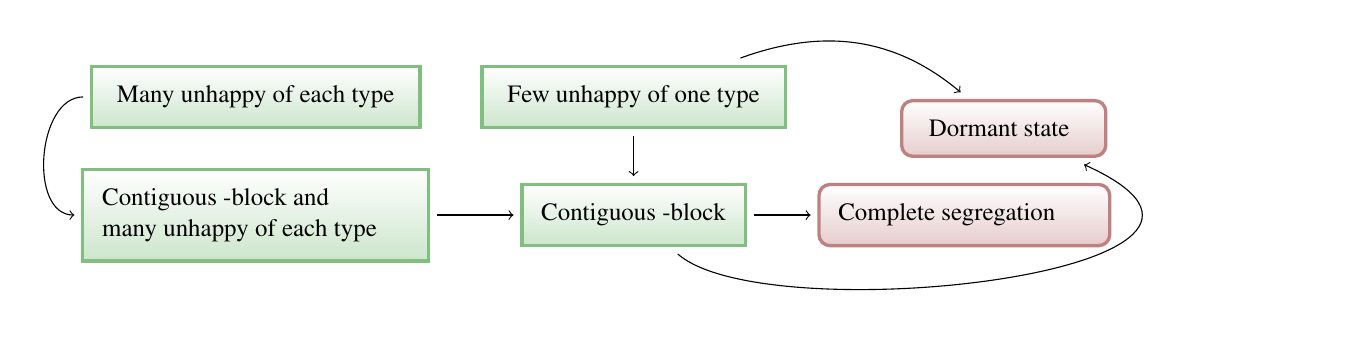
\begin{tikzpicture}[
main/.style={rectangle,  minimum size=6mm, rounded corners, very thick,
draw=red!50!black!50, top color=white, bottom color=red!50!black!20, font=\small},
Nnode/.style={rectangle,  minimum size=6mm, very thick,
draw=green!50!black!50, top color=white, bottom color=green!50!black!20, font=\small },
tnode/.style={rectangle,  minimum size=6mm, rounded corners, very thick,
draw=red!50!black!50, top color=white, bottom color=red!50!black!20, 
 font=\small},
 ttnode/.style={rectangle,  minimum size=6mm, rounded corners, very thick,
draw=yellow!50!black!50, top color=white, bottom color=yellow!50!black!20, 
 font=\small}]
\node (cr) [Nnode,  outer sep=3pt, inner sep=7pt] at (11.3,0.5) {\textrm{Contiguous -block }};
\node (ivr) [main, outer sep=3pt, inner sep=7pt] at (16,1.6) {\parbox{2.1cm}{\hspace{0.1cm}Dormant state\hspace{0.1cm}}};
\node (tivr) [main, outer sep=3pt, inner sep=7pt] at (15.5,0.5) {\parbox{3.2cm}{Complete segregation}};
\node (fvr) [Nnode, outer sep=3pt, inner sep=7pt] at (11.3,2) {\textrm{\ Few unhappy of one type\ \ }};
\node (kr) [Nnode, outer sep=3pt, inner sep=7pt] at (6.5,2) {\textrm{\ Many unhappy of each type\ \ }};
\node (bi) [Nnode, outer sep=3pt, inner sep=7pt] at (6.5,0.5) {\parbox{3.9cm}{Contiguous -block and\\ 
many unhappy of each type}};
\draw [->] (cr) --  (tivr); 
\draw [->] (fvr) to [in=140, out = 20]  (ivr); 
\draw[->]  (cr) .. controls (13,-1) and (20, -0.2) .. (ivr); 
\draw [->] (bi) -- (cr) ; 
\draw [->] (fvr) -- (cr); 
\draw [->] (kr) to [in=180, out = -180] (bi); 
\end{tikzpicture}}
\centering
\caption{The path to a dormant state or complete segregation when .}
\label{fig:skewstratcomd}
\end{figure}



\subsection{Accessibility of dormant states and complete segregation}\label{subse:accdorcose}
We show  the case of Theorem \ref{th:complsegm} where  and
. This argument consists of two parts. First, we show that in this case
with high probability the initial state is such that
every state with the same number of -nodes has unhappy nodes of both types (i.e.\ it is not dormant).
Hence under these conditions, no accessible state is dormant.
The second part consists of showing that from every state there is a sequence of transitions to either a dormant state 
or complete segregation. Moreover the latter fact holds in general, for any values of , so it can be reused for the case when
, in Section \ref{se:recomsehaca}. This latter case is more challenging, 
as it can be seen that there are permutations of the initial state which are dormant.
\begin{lem}[Existence of unhappy nodes]\label{coro:exiunhangen}
Suppose that ,   and  is sufficiently large.
Then for every  and
all sufficiently large , every state of the process
 has more than  unhappy -nodes.
If in addition , every state also has 
more than  unhappy -nodes.
\end{lem}

Given , by the law of large numbers with high probability 
(tending to 1, as  tends to infinity)
 will be arbitrarily close to . 
Hence we may deduce the absence of dormant states
(with high probability) in the case that .
\begin{coro}[Absence of dormant states when  and ]\label{coro:absdormst.g}
If  and   then
with high probability none of the accessible states of
the process 
is dormant.
\end{coro}

It remains to show the accessibility of either a dormant state or
complete segregation, from any state of the process.
An inductive argument can be used in order to prove this fact.


\begin{lem}[Complete segregation or dormant state]\label{coro:inevcompsegd}
From any state of the process  with 
there exists a series of transitions to complete segregation or to a dormant state.
\end{lem}

Here is a sketch of the proof.
If  the mixing index is strictly decreasing through the transitions, so it is immediate
that the process will reach a dormant state (indeed, 0 is a lower bound for the mixing index).
For the case where  (which we assume for the duration of this discussion) we can argue
inductively, in four steps. 
An interval of nodes of the same type is called a {\em contiguous block}. 
First we show that
from a stage with few unhappy nodes of one type (here  is a convenient upper bound of
what we mean by `few', which is by no means optimal) there is a series of transitions which lead to either
a state with a contiguous block of length  or a dormant state.
Second, 
from a state with a contiguous block of length 
there is a series of transitions to complete segregation or to a dormant state.
Third,
any state which has at least  unhappy nodes of each type,
there is a series of transitions to a state with a contiguous 
block of length at least .
Finally 
from a state that has a contiguous block  of length 
and at least  unhappy nodes of opposite type from the block,  there is a series of
transitions to a state with a contiguous block  of length .
The combination of these four statements constitutes a strategy for arriving to a dormant state or
a state of complete segregation, from any given state.
We illustrate this strategy in Figure \ref{fig:skewstratcomd}, where
two arrows leaving a node indicate that at least one of these routes are possible.

 \begin{figure} 
\centering\includegraphics[scale=0.36]{./circle.png}
\caption{The evolution of the infected area when .}\label{fig:cicle_slides}
\end{figure}  


\section{Reaching complete segregation \texorpdfstring{when  and  }{in the hard case}}\label{se:recomsehaca}
This case of Theorem \ref{th:complsegm} is challenging because we need to show that the process avoids accessible dormant states, until it reaches a {\em safe state}
i.e.\ a state from which no dormant state is accessible.
The reason for this avoidance is (in contrast with the case  of Section \ref{subse:accdorcose}) 
the dynamics of the process with the given parameters.
The methodology we use is based on a martingale argument, which involves a great deal of the analytical tools 
(e.g.\ the metrics of social welfare) and their properties that were developed in the previous sections.
Having shown that dormant states are avoided until the process reaches a safe state, Lemma \ref{coro:inevcompsegd} gives
Theorem \ref{th:complsegm} (for the case where  and  ). An overview of this argument is given in Figure \ref{fig:dysimpleskads}.

\subsection{The persistence of large contiguous \texorpdfstring{}{beta}-blocks}\label{se:persist}
According to our plan, we wish to establish the existence of unhappy nodes of both types until a safe state is reached.
By Lemma \ref{coro:exiunhangen}, we do not have to worry about the existence of unhappy -nodes. One device that guaranties the  existence of
unhappy -nodes is a contiguous block of -nodes, of length at least . 
Such a block exists in the initial random state (with high probability). One way to argue for its preservation in subsequent stages is to consider the 
ratio of the unhappy nodes of the two types. 
Even more relevant is the ratio between the number of unhappy -nodes, 
and the number of -nodes which are not just unhappy, but actually sufficiently unhappy that they can swap with any unhappy -node.

\begin{defi}[Very unhappy -nodes]\label{de:veryunhapy}
Given a stage of the process, a node of type  is very unhappy if
there are at least  nodes of type  in its neighbourhood.
The number of very unhappy -nodes is denoted by .
\end{defi}

In the case that we study ( and  ) 
initially, the number of very unhappy -nodes is  while the
number of unhappy -nodes is .
The following lemma says that as long as this imbalance is preserved, it is very likely that a
sufficiently long contiguous block of -nodes is preserved.
\begin{lem}[Persistent \texorpdfstring{}{beta}-block]
\label{le:persistb}
Consider the process
 with   
and let  be the least stage where
the ratio between the very unhappy -nodes and the unhappy -nodes
becomes less than  (putting  if no such stage exists). Then with 
high probability there is a -block of length  at all
stages  of the process. 
\end{lem}

Since a -block of length at least  is a
guarantee for unhappy -nodes, we get the following corollary.

\begin{coro}[Conditional existence of unhappy -nodes]\label{le:percosistb}
Under the hypotheses of Lemma \ref{le:persistb}, 
with high probability 
there are unhappy -nodes at 
all stages  of the process.
\end{coro}

It remains to construct an elaborate martingale argument in order to show that 
the imbalance between  and 
persists for a sufficiently long time (until the process reaches a safe state). 




\subsection{Infected area view of the Schelling process}\label{subse:infareaview}
In the case of unbalanced happiness (i.e.\ when , , see Table \ref{ta:validptwocasesnadcorr})
the unhappy -nodes are initially very rare, so the interesting activity (namely -to- swaps) occurs
in small intervals of the entire population (at least in the early stages). 
These intervals contain the unhappy -nodes, and gradually expand, while outside these intervals
all -nodes are very unhappy. Figure \ref{fig:biasplot}  
shows the development of this process, where the height of the nodes (perpendicular lines) is proportional to
the number of -nodes in their neighborhood and the horizontal black line denotes the 
threshold where an -node  becomes unhappy.
Hence nodes with high proportion of -nodes in their neighbourhood
will be higher than the nodes with low proportion of -nodes in their neighbourhood. 
The three horizontal bars are snapshots of the process, and show
cascades forming, originating from the initially unhappy -nodes. 
Figure \ref{fig:cicle_slides} 
shows the same process, with the current state in the outer circle, and with swaps represented by a
dot at a distance from the center which is proportional to the stage where the swap occurred.
These cascades that spread the unhappy -nodes are due to the following domino effect. An unhappy 
-node moves out of a neighbourhood, thus reducing the number of -nodes in that interval. This
in turn often makes another -node in the interval unhappy, which can move out at a latter stage, thus
causing another -node nearby to be unhappy, and so on.
The expanding intervals are the {\em infected segments} which start their life as {\em incubators}.
For the sake of simplicity, we omit the formal definitions of these notions, which can be found in the appendix.
Roughly speaking,  incubators are a small intervals that surround  the unhappy -nodes in the initial state.
Moreover they are defined in such a way that, every -node that is outside the incubators is {\em very unhappy}
in the initial state.
During the process, as we discussed above, these expand into larger {\em infected segments}, so that at each stage
every unhappy -node is inside an infected segment.
The union of all infected segments is called the 
{\em infected area}. At any stage, every -node outside the infected area is {\em very unhappy}
and every -node outside the infected area is happy.
It is not hard to show that if , the probability that a node belongs to an incubator is
. Hence with high probability  
 the number of incubators as well as the number of nodes belonging to incubators
 of the process  is .


\begin{figure}\scalebox{0.7}{
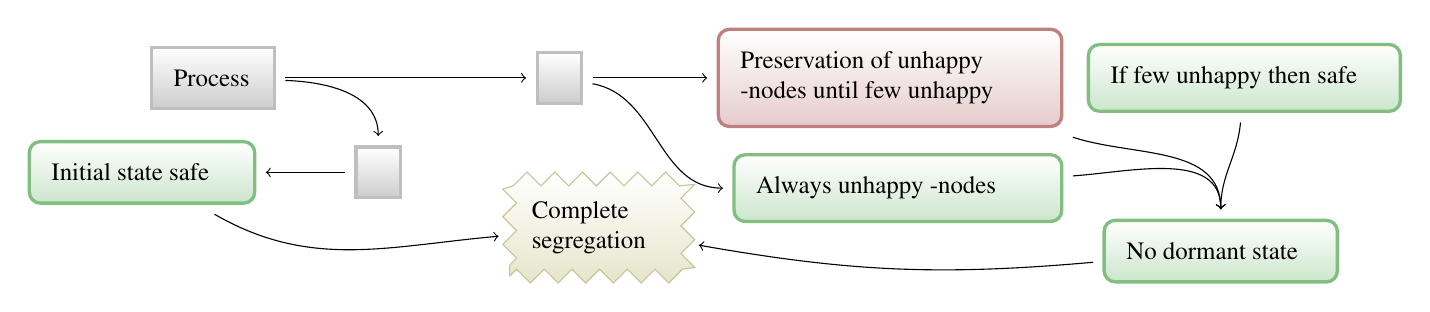
\begin{tikzpicture}[
Nnode/.style={rectangle, rounded corners, minimum height=4mm, very thick, 
draw=green!50!black!50, top color=white, bottom color=green!50!black!20, font=\small },
tnode/.style={rectangle, rounded corners, very thick,
draw=red!50!black!50, top color=white, bottom color=red!50!black!20, font=\small},
pnode/.style={rectangle, very thick,
draw=white!50!black!50, top color=white, bottom color=white!50!black!40, font=\small}]
 \node (Npreserv) [Nnode,  outer sep=4pt, inner sep=8pt] at (7.8,2) {\parbox{3.4cm}{
If few unhappy then safe}};
 \node (Nbreakth) [Nnode,  outer sep=4pt, inner sep=8pt] at (7.5,-0.2) {\parbox{2.4cm}{
 No dormant state}};
 \node (Nunbala) [tnode,  outer sep=4pt, inner sep=8pt] at (3.3,2) {\parbox{3.8cm}{Preservation
 of unhappy\\ -nodes until few unhappy}};
 \node (Nhard) [pnode,  outer sep=4pt, inner sep=8pt] at (-0.9,2) {\parbox{1.3cm}{}};
 \node (Ninitsafe) [Nnode,  outer sep=4pt, inner sep=8pt] at (-6.2,0.8) {\parbox{2.3cm}{Initial state
 safe}};
 \node (Nalwunhab) [Nnode,  outer sep=4pt, inner sep=8pt] at (3.4,0.6) {\parbox{3.6cm}{Always 
unhappy -nodes}};
 \node (Nprocess) [pnode,  outer sep=4pt, inner sep=8pt] at (-5.3,2) {\parbox{1cm}{Process}};
 \node (Neasy) [pnode,  outer sep=4pt, inner sep=8pt] at (-3.2,0.8) {\parbox{1.4cm}{}};
\node (Ncomplete) [draw=yellow!50!black!50, font=\small, top color=white, bottom color=yellow!50!black!20, decorate, decoration=zigzag, 
outer sep=4pt, inner sep=8pt] at (-0.4,0.1) {\parbox{1.7cm}{Complete segregation}};
\draw [->, in = 90, out=-2] (Nprocess) to (Neasy);
\draw [->] (Neasy) to (Ninitsafe);
\draw [->] (Nprocess) to (Nhard);
\draw [->, in = 180, out=-10] (Nhard) to (Nalwunhab);
\draw [->] (Nhard) to (Nunbala);
\draw [->, in = 90, out=4] (Nalwunhab) to (Nbreakth);
\draw [->, in = 90, out=-95] (Npreserv) to (Nbreakth);
\draw [->, in = 90, out=-18] (Nunbala) to (Nbreakth);
\draw [->,  in = -10, out=185] (Nbreakth) to (Ncomplete);
\draw [->,  in = 185, out=-30] (Ninitsafe) to (Ncomplete);
\end{tikzpicture}}
\centering
\caption{The logic of the proof that if , with high probability
the process reaches complete segregation.}\label{fig:dysimpleskads}
\end{figure}

It turns out that the number of unhappy -nodes in an interval of nodes, is conveniently bounded
in terms of the number of -nodes in the interval.
This means that  if the number of -nodes in the infected area remains , then
the number of unhappy -nodes in the infected area also remains .
In order to give a clear sketch of the argument depicted in Figure \ref{fig:dysimpleskads}
(for the current case when  and )
let us define the global variables in Table \ref{ta:pranvarinfarfa2}
(for the current discussion we will not be concerned with  or its definition).
Note that Since .
A combinatorial argument can be used in order to show that .
Hence 

By \eqref{eq:finalumixkrel}  we know that a stage where the number of unhappy nodes
is less than  is a safe stage.
Hence we wish to show that (with high probability) 
the process will arrive at a stage where  each of the three
summands in \eqref{eq:uscsgszs} are at most
. We know that  
can be bounded appropriately. Our main argument will show
how to obtain a similar bound for . 
Note that  plays a different role,
since it is initially large and shrinks monotonically (as the infected area expands monotonically). 
In order to find a stage where  becomes sufficiently small, it is instructive to consider what is a typical swap
in the process.
At the start of the process the infected area is a very small proportion of the
entire ring. The vast majority of unhappy -nodes occur outside
the infected area, while all unhappy -nodes are inside the infected area.
It follows that with high probability a 
swap will involve an -node in the infected
area and a -node outside the infected area. A {\em bogus swap} is a swap is one that is not of this kind.

\begin{defi}[Bogus swaps]
A swap
which involves a -node 
currently inside the infected area is called bogus. 
Given an infected segment , a bogus swap in  is a
swap that moves an -node into .
\end{defi}

\begin{table}\caption{Random variables indicating the number of certain nodes in 
infected area at stage  of the 
process.}\label{ta:pranvarinfarfa2}
\colorbox{black!10}{\arrayrulecolor{green!50!black} 
\begin{tabular}{cl}\toprule
{\bf\small }  &   \textrm{\small -nodes in infected area}\1ex]
{\bf\small }  &   \textrm{\small Anomalous nodes in infected area}  \1ex]
{\bf\small }  &   \textrm{\small -nodes outside infected area.}  \1ex]  
\bottomrule \end{tabular} } 
\centering
\end{table}

Note that any swap which is not bogus, reduces  by at least 1. Hence if we show that the bogus swaps have
small probability throughout a significant part of the process, we can ensure that  becomes sufficiently small.
In order to be more precise,
recall the stopping time 
from Lemma \ref{le:persistb}.
We introduce a few more stopping times, all of which 
will turn out to be earlier than  (with high probability). These  
basically concern the satisfaction of conditions which will ensure that 
the mixing index is sufficiently low as to guarantee a safe state. 
By \eqref{eq:finalumixkrel} 
we have 
and in order to ensure a safe state (by Lemma \ref{le:mixindorsta}) 
we want . 
So we want  at some stage of the process.
Let  be 
the first stage which satisfies this condition.
Similarly, consider the stopping times  of 
the second part of Table \ref{ta:validprglobbouatd} (for simplicity, we will not consider  in the present discussion).
We use an elaborate martingale argument in order to show the following.

\begin{lem}[Bounding the -nodes in the infected area]\label{le:inthzbouwe}
If  and , 
with high probability we have  and  for all .
\end{lem}

This lemma in combination with Corollary \ref{le:persistb} 
implies that .
Hence every stage up to  involves a swap.
Then it follows from the second clause of Lemma \ref{le:inthzbouwe}  
that  (since  is reduced by at least 1 
at every non-bogus swap).
Hence by \eqref{eq:uscsgszs} we have established (with high probability) the existence of a stage  such that



Hence  by \eqref{eq:finalumixkrel} we have ,
which means that by stage  a safe state has been reached.
Then by Corollary \ref{coro:inevcompsegd} the process will reach complete segregation, with probability
.

\begin{coro} [Safe state arrival]
Suppose that . Then with high probability
the process   reaches a safe state by stage , and eventually complete segregation.
\end{coro}

This argument (with the full details given in Section \ref{se:prelim})
concludes the proof of Theorem \ref{th:complsegm} for the case .
It remains to deal with the case .






\begin{table}\caption{Likelihood of various properties 
in the initial configuration under certain conditions, when  and }
\label{ta:vlikelyghd}
\colorbox{black!10}{\arrayrulecolor{green!50!black} 
 \begin{tabular}{ccccc}
 {\bf\small Property}&  & {\bf\small Probability} &  {\bf\small Distribution}& {\bf\small Likelihood}\1ex]
{\small Unhappy -node}  & \hspace{0.3cm} & {\small } &{\small }\hspace{0.5cm} &{\small always rare}\
\Pstab=\proba{Z_{\textrm{stab}}\geq (2w+1)\tau}
\hspace{1cm}
\textrm{and}
\hspace{1cm}
\Punhap\geq 
\proba{Z_{\textrm{unhap}}\geq 2w(1-\tau)}.
1ex]
 \cmidrule{1-4}
{\small  \hspace{0.1cm}}&&
{\small } & 
{\small  \hspace{0.2cm}and \hspace{0.2cm}}\1ex]
\end{tabular}}
\centering
\end{table}

The intuition here is that, if the unhappy -nodes are much more rare than the
stable -stable intervals (i.e.\  if )  then it is very likely that unhappy
-nodes are enclosed in small intervals which are guarded by -stable intervlas. This means that
the familiar cascades that can be caused by the eviction of an unhappy -node are bound to be contained in small
areas of nodes. The very definition of stable intervals ensures that such cascades cannot pass through them. Hence the condition
  guarantees that any -to- swaps are contained in small areas of nodes of total size .
 Due to the monotonicity of the mixing index, this means that there can only be at most 
  swaps in this case.
 
The second item in Figure \ref{fig:red_3D_tr} shows the probabilities  (for )
with respect to . We see that for points away from , the surface  is above , 
and there is a threshold curve beyond which the opposite relationship is established.
Using basic results about the tail of the binomial distribution, and Stirling's approximation
we can derive the following sufficient condition for :

The third item of Figure \ref{fig:red_3D_tr}
is a representation of  in the space, up to where
it becomes negative, at which point we project it on the plane.
The values of  that we are interested correspond to points
on the plane, outside the collapsed area.
This boundary (a curve) is more clear in the first 
item of Figure \ref{fig:red_3D_tr} which is the projection of the
surface to the plane, with different colours indicating the points
which make  positive or negative.
This boundary can be simplified (with slight loss of generality) if we consider the line
that passes from the two points where the boundary curve intersects the lines  and .
Hence if , we are in the stable region, which shows a clause of Theorem \ref{th:complsegm}. 
Note that both of the partial derivatives of  are negative 
when .
If we fix  then the largest value of  that keeps 
is the solution () of the first equation
of Table \ref{ta:constantthresint}. 
Hence we may conclude that
if   
and  then 

for some .
We can also look for the largest square that is contained 
in the large area of the first item of Figure \ref{fig:red_3D_tr} (where the process is static).
The edge of this square is given in Table \ref{ta:constantthresint}.
Hence if  
then 
for some .


We have one last observation to make about the function .
If we let do not restrict the values of  then we wish to
find the values of  such that . According to the properties of
 (in particular its negative derivative on ), 
these are all the positive numbers which are less than the limit 
(which is also an infimum)


Hence 
we may conclude that
if 
and  
then 
for some .
This concludes the proof of the second clause 
of Theorem \ref{th:complsegm}.
 




\newpage

\begin{thebibliography}{CMGP13}

\bibitem[BELP14]{BELschel13}
G.~Barmpalias, R.~Elwes, and A.~Lewis-Pye.
\newblock Digital morphogenesis via {S}chelling segregation.
\newblock In {\em 55th Annual IEEE Symposium on Foundations of Computer
  Science}, Oct. 18-21, Philadelphia, 2014. FOCS 2014.

\bibitem[BELP15]{BELtipl13}
G.~Barmpalias, R.~Elwes, and A.~Lewis-Pye.
\newblock {Tipping Points in 1-Dimensional Schelling Models with Switching
  Agents}.
\newblock {\em J.\ Stat.\ Phys.}, 158:806--852, 2015.

\bibitem[Ber12]{Bertin}
E.~Bertin.
\newblock {\em A Concise Introduction to the Statistical Physics of Complex
  Systems}.
\newblock Springer Briefs in Complexity. Springer, Springer Berlin Heidelberg,
  2012.

\bibitem[BIKK12]{brandt:an}
C.~Brandt, N.~Immorlica, G.~Kamath, and R.~Kleinberg.
\newblock An analysis of one-dimensional {S}chelling segregation.
\newblock In {\em STOC '12: Proceedings of the 44th symposium on Theory of
  Computing}, pages 789--804, 2012.

\bibitem[BMR14]{DBLP:conf/soda/BhaktaMR14}
P.~Bhakta, S.~Miracle, and D.~Randall.
\newblock Clustering and mixing times for segregation models on
  {}.
\newblock In {\em Proceedings of the Twenty-Fifth Annual {ACM-SIAM} Symposium
  on Discrete Algorithms, {SODA} 2014, Portland, Oregon, USA, January 5-7,
  2014}, pages 327--340, 2014.

\bibitem[Bolon]{Bollobas_random}
B.~Bollob\'{a}s.
\newblock {\em Random Graphs}.
\newblock Cambridge Studies in Advanced Mathematics 73. Cambridge University
  Press, Trinity College, Cambridge and University of Memphis, 2001, Second
  Edition.

\bibitem[CACP07]{CACP07}
R.~Conte, G.~Andrighetto, M.~Campenn\`{i}, and M.~Paolucci.
\newblock Emergent and immergent effects in complex social systems.
\newblock In {\em Proceedings of AAAI Symposium, Social and Organizational
  Aspects of Intelligence}, Washington DC, 2007. Association for the
  Advancement of Artificial Intelligence.

\bibitem[CF08]{CF}
W.\ Clark and M.\ Fossett.
\newblock Understanding the social context of the {S}chelling segregation
  model.
\newblock {\em Proceedings of the National Academy of Sciences}, 11:4109--4114,
  2008.
\newblock col.\ 105.

\bibitem[CFL09]{RevModPhys.81.591}
C.~Castellano, S.~Fortunato, and V.~Loreto.
\newblock Statistical physics of social dynamics.
\newblock {\em Reviews of Modern Physics}, 81:591--646, 2009.

\bibitem[Cla91]{Clarkdem}
W.\ Clark.
\newblock Residential preferences and neighborhood racial segregation: A test
  of the {S}chelling segregation model.
\newblock {\em Demography}, 28:1--19, 1991.

\bibitem[CM11]{howtop}
P.~Collard and S.~Mesmoudi.
\newblock How to prevent intolerant agents from high segregation?
\newblock In {\em Advances in Artificial Life (ECAL 2011), Paris, France (T.
  Lenaerts et al., eds.), Cambridge, MA: MIT Press}, 2011.

\bibitem[CMGP13]{MF}
P.~Collard, S.~Mesmoudi, T.~Ghetiu, and F.~Polack.
\newblock Emergence of frontiers in networked {S}chelling segregationist
  models.
\newblock {\em Journal of Complex Systems}, 22, 2013.

\bibitem[DCM08]{DM}
L.~Dall'Asta, C.~Castellano, and M.~Marsili.
\newblock Statistical physics of the {S}chelling model of segregation.
\newblock {\em Journal of Statistical Mechanics: Theory and Experiment}, 7,
  2008.

\bibitem[dSGL07]{deSmith:2007:GAC:1557282}
Michael~J. de~Smith, Michael~F. Goodchild, and Paul~A. Longley.
\newblock {\em Geospatial Analysis: A Comprehensive Guide to Principles,
  Techniques and Software Tools}.
\newblock Troubador Publishing, 2nd edition, 2007.

\bibitem[EA96]{epstein1996growing}
J.M. Epstein and R.~Axtell.
\newblock {\em Growing Artificial Societies: Social Science from the Bottom
  Up}.
\newblock A Bradford book. Brookings Institution Press, 1996.

\bibitem[Fos06]{FMpref}
M.~Fossett.
\newblock Ethnic preferences, social distance dynamics, and residential
  segregation: Theoretical explorations using simulation analysis.
\newblock {\em Journal of Mathematical Sociology}, 30:185--273, 2006.

\bibitem[GB02]{Gilbert14052002}
N.~Gilbert and S.~Bankes.
\newblock Platforms and methods for agent-based modeling.
\newblock {\em Proceedings of the National Academy of Sciences}, 99(suppl
  3):7197--7198, 2002.

\bibitem[Hay13]{Hayes}
B.~Hayes.
\newblock The math of segregation.
\newblock {\em {American Scientist}}, 101(5):338--341, 2013.

\bibitem[HCSB11]{heppenstall2011agent}
A.J. Heppenstall, A.T. Crooks, L.M. See, and M.~Batty.
\newblock {\em Agent-Based Models of Geographical Systems}.
\newblock Springer Netherlands, 2011.

\bibitem[LG09]{GVN}
J.-P.~Nadal L.~Gauvin, J.~Vannemenus.
\newblock Phase diagram of a {S}chelling segregation model.
\newblock {\em European Physical Journal B}, 70:293--304, 2009.

\bibitem[Mou10]{mousavi}
Nima Mousavi.
\newblock How tight is {C}hernoff bound?, 2010.
\newblock Draft which is available for download at
  http://ece.uwaterloo.ca/nmousavi.

\bibitem[\'{O}08]{GO}
G.\ \'{O}dor.
\newblock {Self-organising, two temperature Ising model describing human
  segregation}.
\newblock {\em International journal of modern physics C}, 3:393--398, 2008.

\bibitem[PW01]{PW}
M.\ Pollicott and H.\ Weiss.
\newblock {The dynamics of {S}chelling-type segregation models and a non-linear
  graph Laplacian variational problem}.
\newblock {\em Adv. Appl. Math.}, 27:17--40, 2001.

\bibitem[Sch69]{TS1}
T.~C. Schelling.
\newblock Models of segregation.
\newblock {\em The American Economic Review}, 59(2):488--493, 1969.

\bibitem[Sch71a]{TS71a}
T.C. Schelling.
\newblock Dynamic models of segregation.
\newblock {\em Journal of Mathematical Sociology}, 2:143--186, 1971.

\bibitem[Sch71b]{TS71b}
T.C. Schelling.
\newblock On the ecology of micromotives.
\newblock {\em The Public Interest}, 25:61--98, 1971.

\bibitem[Sch78]{TS2}
T.~C. Schelling.
\newblock {\em Micromotives and Macrobehavior}.
\newblock New York, Norton, 1978.

\bibitem[Sch07]{Martijn2007}
M.C. Schut.
\newblock Scientific handbook for simulation of collective intelligence.
\newblock http://www.sci-sci.org, 2007.

\bibitem[Slu77]{sludche}
E.~V. Slud.
\newblock Distribution inequalities for the binomial law.
\newblock {\em Ann. Probab.}, 5:404--412, 1977.

\bibitem[SS07]{SS}
D.~Stauffer and S.~Solomon.
\newblock Ising, {S}chelling and self-organising segregation.
\newblock {\em The European Physical Journal B - Condensed Matter and Complex
  Systems}, 57(4):473--479, 2007.

\bibitem[SSD00]{SandSDo}
R.~Sander, D.~Schreiber, and J.~Doherty.
\newblock Empirically testing a computational model: The example of housing
  segregation.
\newblock In {\em Proceedings of the Workshop on Simulation of Social Agents:
  Architectures and Institutions}, pages 108--115, Lexington, MA, 2000.
  Lexington Books.

\bibitem[Wil99]{NetLogo}
U.~Wilensky.
\newblock {\em NetLogo Models Library: Sample Models/Social Science}.
\newblock NetLogo. http://ccl.northwestern.edu/netlogo, Center for Connected
  Learning and Computer-Based Modelling, North-Western University. Evanston,
  IL., 1999.

\bibitem[Y{\"O}09]{yilmaz2009agent}
L.~Yilmaz and T.~{\"O}ren.
\newblock {\em Agent-Directed Simulation and Systems Engineering}.
\newblock Wiley Series in Systems Engineering and Management. Wiley, 2009.

\bibitem[You98]{HY}
H.P.\ Young.
\newblock {\em Individual Strategy and Social Structure: An Evolutionary Theory
  of Institutions}.
\newblock {Princeton University Press}, Princeton, NJ, 1998.

\bibitem[Zha04a]{JZ1}
J.\ Zhang.
\newblock A dynamic model of residential segregation.
\newblock {\em Journal of Mathematical Sociology}, 28(3):147--170, 2004.

\bibitem[Zha04b]{JZ2}
J.\ Zhang.
\newblock Residential segregation in an all-integrationist world.
\newblock {\em Journal of Economic Behavior \& Organization}, 54(4):533--550,
  2004.

\bibitem[Zha11]{JZ3}
J.\ Zhang.
\newblock Tipping and residential segregation: A unified {S}chelling model.
\newblock {\em Journal of Regional Science}, 51:167--193, 2011.

\end{thebibliography}

\newpage


\section{Appendix}\label{se:prelim}
In this section we provide supplementary material to the main part of the paper. 
This includes mainly proofs of the claims we made towards the proof of our main theorem, but also
additional introductory material, figures, tables and mathematical background.
The structure of this supporting material follows the presentation of the main part of the paper.

\subsection{Schelling models}\label{ssub:varschel}
The definition of the Schelling model in Section \ref{def:modseg} is rather standard, close to
the spacial proximity model from  \cite{TS1, TS71a}  and identical to
the model studied in \cite{brandt:an, BELschel13}. 
Most significantly, it is an unperturbed Schelling model, where agents cannot
make moves that are detrimental to their welfare.
We have already remarked in the introduction
that various more realistic-looking rigorously analysed perturbed versions of the model 
in the literature (such as \cite{JZ1}) actually force `regularity' on the process, which
makes it fit an already existing methodology 
(such as Markov chains with a unique stationary distribution, 
or with properties that guarantee stochastically stable states).
Even if we commit to the absence of perturbations in the model, 
it is possible to add complications to the simple dynamics defined in
Section \ref{def:modseg}. For example, the agents
may take into account the distance they need to travel before they move.
However it is the simplicity of the original Schelling model,
contrasted by  the complexity of the analysis required to specify its behaviour
(as demonstrated in \cite{brandt:an, BELschel13}) 
that make this topic fundamental and interesting.

Under the above requirement for simplicity and proximity to the original model,
there remain a number of ways that the model can be altered or generalised.
For example, note that in the case that  in the model of
Section  \ref{def:modseg}, two nodes may swap although the number of
same-type nodes in their neighbourhoods remain the same after the swap.
One may alternatively require that for such a swap, the corresponding
numbers of same-type nodes in the neighbourhoods increase
(note that such a modification would not make a difference if ).
Our choice on this issue follows Brandt, Immorlica, Kamath, and Kleinberg in
\cite[Section 2]{brandt:an}.
One generalisation, considered in \cite{BELtipl13}, is to allow
different tolerance thresholds for the two types of
individuals. Another generalization, already present in \cite{TS1}, is to introduce a number
of vacancies, i.e.\ to allow the total number of individuals to 
be smaller than the number of sites. 
We could also alter the dynamics. Instead
of switching two chosen individuals at each stage, we could merely choose {\em one}
individual and change his type. Such an action may be 
interpreted as the departure of the individual to some external location and the arrival of an 
individual of the opposite type at the site that has just become available. 
Model with this dynamics are often said to have {\em switching agents}
(see \cite{BELtipl13}, where such a model was analysed) as opposed to the 
{\em swapping agents} of the model of Section \ref{def:modseg}. 

It is worth pointing out that the Schelling model with switching agents
is closely related to the spin-1 models used to analyse phase transitions in physics, and in
particular the Ising model. Indeed, in the Ising model (originally introduced in order to explain
ferromagnetism in the context of temperature) a system of atomic nuclei interact with an 
auxiliary `heat bath' which affects their spin. Such connections have been analysed by many authors
(see for example \cite{SS,DM,PW,GVN,GO}), where the dynamics is based on
the Boltzmann distribution on the set of possible configurations. A rough analogy between
the two models is that `energy'  corresponds to  some measure of the mixing of types
(see the definition of the mixing index for the Schelling model below) and `temperature' 
corresponds to the intolerance parameter  (as least insofar phase transitions refer to
varying values of the temperature or ). On the other hand, 
the Schelling model with closed dynamics has a counterpart in the
Ising model with Kawasaki dynamics.

\subsection{Objectives of the analysis of the unperturbed model and related work}
\label{sub:knownressch}
\label{se:1Dmorphojob}
We use the notation of Section \ref{def:modseg}, so that 
the symbol  always means the population
variable of the process, and  always is the parameter of the process which
determines the length of the neighbourhood of nodes. Similarly, 
always refer to the parameters of the Schelling process.

In Section \ref{se:accesscomplseg} we show that,
with probability one, the process 
 either reaches complete segregation or
it reaches a dormant state.
In the second case, we wish to 
determine the extent of segregation in the dormant state.
In view of the large number of states that the process may have
(most of them `random') a question arrises as to how to classify or even
talk precisely about different states that may be the outcome of the process.
Brandt, Immorlica, Kamath, and Kleinberg noticed in \cite{brandt:an} that, 
at least in the case  that they considered, 
the extent of the segregation that occurs in the final state
depends crucially on . In fact, they showed that
the dependence on  is `polynomial'.
We may say that
a state is regarded as {\em polynomial segregation} if, with high probability
a randomly chosen node belongs to a contiguous block of size that is proportional to 
the value of a polynomial on . A similar definition applies to 
{\em exponential segregation}. These two notions turn out to provide 
a very useful language for explaining the eventual outcome of the Schelling process.
A full characterization (extending the work of Brandt, Immorlica, Kamath, and Kleinberg 
\cite{brandt:an}) of the asymptotic behaviour of the process 
for  and  was provided by the authors in \cite{BELschel13}
in terms of polynomial and exponential segregation, as well as static processes.
Intuitively, a random state is non-segregated, while polynomial 
and exponential segregation correspond to highly non-random states.
\begin{table}
\colorbox{black!10}{\arrayrulecolor{green!50!black}
\begin{tabular}{l|cccc}
\toprule
{\small\bf Intolerance}& {\small } & {\small  } & 
{\small  }&{\small  } \\label{eq:gjrisrig}
\sum_{j<n_{\beta}} \beta_j^{\alpha} = \sum_{i<n_{\alpha}} \alpha_i^{\beta}.
\label{eq:twosumeqs}
\sum_{i<n_{\alpha}} \alpha_i^{\alpha} + 
\sum_{i<n_{\alpha}} \alpha_i^{\beta} = 
(2w+1)\cdot n_{\alpha} \hspace{0.5cm}\textrm{ and }\hspace{0.5cm}
\sum_{j<n_{\beta}} \beta_j^{\beta} + \sum_{j<n_{\beta}} \beta_j^{\alpha} 
= (2w+1)\cdot n_{\beta}.
\label{eq:mixindtoblock}
\sum_{i<n_\beta} \beta_i^{\alpha} \leq w(w+1) \cdot \mathtt{k}_{\beta},\hspace{0.4cm}\textrm{where  is the number of maximal -blocks.}

\mix \leq w\cdot (w+1) \cdot \mathtt{k}_{\beta} \leq w\cdot (w+1) \cdot \unhap

\unhap_{\alpha}\cdot (1-\tau)(2w+1)\leq  \mix\hspace{0.5cm}
\textrm{and}\hspace{0.5cm}\unhap_{\beta}\cdot (1-\tau)(2w+1)\leq \mix

\mix \leq w\cdot (w+1) \cdot \mathtt{k}_{\beta} \leq w\cdot (w+1) \cdot \unhap
\leq \mix\cdot \frac{2w(1+1/w)}{(1-\tau)(2+1/w)}< \mix\cdot \frac{2w}{1-\tau}

\frac{1}{w}\cdot \frac{\mix}{w+1} \leq \mathtt{k}_{\beta} \leq\unhap< \frac{2}{1-\tau}\cdot \frac{\mix}{w+1}

\sum_{s\in[ r/t_0, m)} e^{-2\delta^2s}\leq 
\frac{e^{-2r\delta^2/t_0}}{1-e^{-2\delta^2}}

\textrm{there exists}\hspace{0.3cm}
q\in \left(\frac{1}{p(k)}, p(k)\right)\hspace{0.4cm}
\textrm{such that}\hspace{0.4cm}
\binom{k}{\ceil{x}}=q\cdot \binom{k}{\floor{x}}.

z'!=q\cdot z\hspace{0.4cm}
\textrm{for some}\hspace{0.4cm}
q\in \left(\frac{1}{r(k)}, r(k)\right).

(z+\delta)^{z+\delta+\frac{1}{2}}=z^z\cdot (z+\delta)^{\delta +\frac{1}{2}}
\cdot \left( 1+\frac{\delta}{z}\right)^z.

(z+\delta)^{z+\delta+\frac{1}{2}}\in \left(z^z\cdot r(k)^{-1},\ z^z\cdot r(k)\right). 

\proba{X_N = h(N)} \ \ \leq \ \ 
\proba{X_N \geq h(N)} \ \ \leq \ \ 
\left( \frac{1}{1-k} \right) \cdot \proba{X_N = h(N)}
\label{eq:coverwIi}
2f(w)M_n \leq |S-\cup_{i<M_n} I_i| < 2f(w)M_n+mf(w)+2f(w).
\label{eq:prob1newis}
\frac{\sum_{i<M_n} Y_i}{M_n}\to 
pmf(w) \hspace{0.4cm}
\textrm{as , with probability 1.}

\frac{\sum_{i<M_n} Y_i +\zeta f(w)\cdot (2M_n+m+2)}{(M_n +\delta) f(w)(m+2)}=
\frac{\frac{\sum_{i<M_n} Y_i}{M_n} +
\zeta f(w)\cdot (2+\frac{m+2}{M_n})}{(1 +\frac{\delta}{M_n}) f(w)(m+2)}

\frac{pm f(w)+2f(w)\zeta}{f(w)(m+2)}=
\frac{pm +2\zeta}{m+2}=
\frac{p +\frac{2\zeta}{m}}{1+\frac{2}{m}}.

\textrm{:\ \ \ \  holds and no node  to the left of
 and at distance at most   satisfies }.

\frac{\rho_n}{\lambda_n}\leq 
\frac{(2\ell+1) \pi_n k_n}{(1-\pi_n)k_n}=
\frac{(2\ell+1) \pi_n}{1-\pi_n}\Rightarrow
\pi_n\geq \frac{\rho_n}{\rho_n+\lambda_n (2\ell+1)}
\label{eq:bouleIm}
|I_m|\leq 2w+1+mw.
\label{eq:vlowbou}
\bias{N_i}\geq (2w+1) (2\tau-1)\hspace{0.5cm}\textrm{and}
\hspace{0.5cm} V_m\geq (m+1)(2w+1) (2\tau-1).
\label{eq:breakvm}
V_m = 2\bias{I_m}-\bias{J^m_1}+\bias{J^m_3} +2\bias{J^m_4}\hspace{0.4cm}\textrm{and}\hspace{0.4cm}
V_m \leq 2\bias{I_m}+2w+\bias{J^m_3}.
\label{eq:jm3unravel}
\bias{J^m_3}< m + \sum_{i=1}^{m-1} (|L_i'|-|R_i'|).

\sum_{i=1}^{m-1} (|L_i'|-|R_i'|)\leq |L_{m-1}'|-|R_{1}'|\leq w.
\label{eq:lowbouthetaimeve}
2\bias{I_m} > (m+1)(2w+1)(2\tau-1)-3w-m.

\bias{I_m}\leq  mw(2\theta_{\ast}-1) + 2w(3\theta_{\ast}-1) +2\theta_{\ast}-1.
\label{finalgthasd}
2m\cdot [2w(\tau-\theta_{\ast})-(1-\tau)]< 
w(12\theta_{\ast}-4\tau+1)  +4\theta_{\ast}-2\tau-1.

n< 3w+1 + w\cdot \frac{w(12\theta_{\ast}-4\tau+1)  +4\theta_{\ast}-2\tau-1}{4w(\tau-\theta_{\ast})-2(1-\tau)}
\label{eq:eqforproai}
e^{-2(y-2w)\delta^2/w}/(1-e^{-2\delta^2})<\epsilon/2.

\probac{X_s>0}{X_s\neq 0}>\frac{2w}{2w+1}> \frac{w}{w+1}+\delta

\textrm{
(a)\hspace{0.2cm}
\hspace{1cm}
(b)\hspace{0.2cm}
\hspace{1cm}
(c)\hspace{0.2cm}
\hspace{1cm}
(d)\hspace{0.2cm}
}

\textrm{ 
\hspace{1cm}and\hspace{1cm}
}

\GG_s\cdot 
\frac{\ZZ_s-\DD_s-2w\cdot \CC}{(\GG_s+\YY_s)\cdot \unhap_{\alpha}(s)}

2w\cdot \frac{\CC\cdot (\GG_s+\YY_s)}{\GG_s\cdot \unhap_{\alpha}(s)}
\label{eq:expecpqzsfs}
E\leq p\cdot (\ZZ_s+w) +
q\cdot (\ZZ_s-1) + (1-p-q)\cdot \ZZ_s = \ZZ_s + wp-q.

2w^2\cdot\CC\cdot\frac{\GG_s+\YY_s}{\GG_s\cdot \unhap_{\alpha}(s)}
\leq \frac{\GG_s}{\unhap_{\alpha}(s)}\cdot \frac{\ZZ_s-\DD_s-2w^2\cdot\CC}{\GG_s+\YY_s}
\hspace{0.5cm}
\textrm{so}
\hspace{0.5cm}
\ZZ_s\geq \DD_s + 2w^2\cdot\CC\cdot\left[1+ \left(1+\frac{\YY_s}{\GG_s}\right)^2\right]
.
\textrm{If  is an enumeration of the -stages, let
 and .}

\textrm{
 for each .}
\label{eq:prob234o}
\parbox{11cm}{in  many -stages  cannot grow by more than .}
\parbox{12cm}{event (c)  has probability  (conditional on ) 
upper bounded by .} 

 \frac{1-q^{w^5/\delta}}{q^{-w\delta}-q^{w^5/\delta}}<
 \frac{1}{q^{-w\delta}}<(w^{3\cdot 5}/n)^{w\delta}
 \label{eq:probbluefis}
\parbox{11cm}{event (d)  has probability (conditional on ) upper bounded by .} 

4w+ 2\frac{w^{2\cdot 5+2}}{n}\cdot w^5\leq 4w+\frac{w^{3\cdot 5+3}}{n}<5w.
\label{eq:ddhola}
 \expeco{\hat{\DD}_{\tau_{s+1}}}{\LL_{\tau_{s}}}{A} \leq  \hat{\DD}_{\tau_{s}} +20w\ \ \ \ \textrm{for all .}

 \expeco{\hat{\DD}_{\tau_{s+1}}}{\LL_{\tau_{s}}}{A} =
 \sum_{j<t} \expeco{\hat{D}_{\tau_{s+1}}(I_j)}{\LL_{\tau_{s}}}{A}
 
\textrm{  for }

 \expec{\hat{\DD}_{\tau_{s+1}}}{\LL_{\tau_{s}}} \leq  \hat{\DD}_{\tau_{s}} +20w\ \ \ \ \textrm{for all .}
\label{eq:ladispe}
\textrm{with probability ,}\ \ \ \ 
\hat{\DD}_{s}< a+ \frac{20s}{w^{4}} \ \ \ \textrm{for all .}

n\cdot \tau\rho/4 < w\cdot \GG_{T_y}< w\cdot 
\frac{\ZZ_{T_y}}{1-\tau}+w^2\cdot \CC
< \frac{n\tau\rho(1-\tau)}{32} + \frac{n\tau\rho}{32}< \frac{n\tau\rho}{16}
\label{eq:bogusprobast}
\textrm{with probability at least ,
at all stages   
we have .}

\GG_{T_y}\leq \GG_0-(1-\epsilon) T_y
\Rightarrow
T_y\leq (\GG_0-\GG_{T_y})/(1-\epsilon)\leq n(\rho+1/8)/(1-\epsilon)<n

\mathtt{U}_{T_g}\leq 
\GG_{T_g} + \YY_{T_g} + \ZZ_{T_g}\leq
\CC(w+1) + \GG_{T_g} + 2\ZZ_{T_g} /(1-\tau)\leq
\frac{3\rho}{4}\cdot\frac{n\tau}{w}<
\frac{n\tau\rho_{\ast}}{w}

with probability .
But  
so the mixing index at stage  is less than
. In other words, , so
by Proposition \ref{prop:maxmixindor} the process at stage  is
in a safe state, with probability more than .
Hence by Corollary \ref{coro:inevcompsegd1}, the process will arrive
to complete segregation 
with probability at least .
\end{proof}





\end{document}